\documentclass[12pt, a4paper]{article}

% PACOTES BÁSICOS
\usepackage[utf8]{inputenc}
\usepackage[brazil]{babel}
\usepackage{geometry}
\usepackage{graphicx}
\usepackage{hyperref}
\usepackage{booktabs} % Para tabelas com visual profissional
\usepackage{listings} % Para blocos de código
\usepackage{xcolor}   % Para cores no código

% CONFIGURAÇÕES
\geometry{a4paper, margin=1in}

% --- Configuração de Cores e Links ---
\hypersetup{
    colorlinks=true,
    linkcolor=blue,
    filecolor=magenta,      
    urlcolor=cyan,
}

% --- Configuração do Pacote Listings para Código ---
\definecolor{codegreen}{rgb}{0,0.6,0}
\definecolor{codegray}{rgb}{0.5,0.5,0.5}
\definecolor{codepurple}{rgb}{0.58,0,0.82}
\definecolor{backcolour}{rgb}{0.95,0.95,0.92}

\lstdefinestyle{mystyle}{
    backgroundcolor=\color{backcolour},   
    commentstyle=\color{codegreen},
    keywordstyle=\color{magenta},
    numberstyle=\tiny\color{codegray},
    stringstyle=\color{codepurple},
    basicstyle=\ttfamily\footnotesize,
    breakatwhitespace=false,         
    breaklines=true,                 
    captionpos=b,                    
    keepspaces=true,                 
    numbers=left,                    
    numbersep=5pt,                  
    showspaces=false,                
    showstringspaces=false,
    showtabs=false,                  
    tabsize=2
}
\lstset{style=mystyle}

% --- INFORMAÇÕES DO DOCUMENTO ---
\title{\textbf{Relatório Técnico Interno: Análise do Projeto de Extração de Dados do ERA5}}
\date{06 de setembro de 2025}

\begin{document}

\maketitle


\hrule
\vspace{12pt}

% --- SEÇÃO 1: RESUMO DO PROJETO ---
\section{Resumo do Projeto}

O projeto consiste em um pipeline para a automação do download de dados de reanálise climática do \textbf{ERA5}, disponibilizados pelo ECMWF através da API do Climate Data Store (CDS). O fluxo de trabalho implementado abrange três etapas principais:

\begin{enumerate}
    \item \textbf{Estudo e Interação com a API do CDS}: O projeto demonstra uma compreensão clara das regras, formatos e limitações da API, como os limites de \textit{fields} por requisição e o tamanho máximo de download, informações cruciais documentadas no \texttt{README.md}.

    \item \textbf{Extração de Dados via Script Python}: Foi desenvolvido o script \texttt{cdsAPI.py}, que automatiza a autenticação, definição de parâmetros (variáveis, área, período) e o download dos dados. O formato de saída padrão é o \textbf{NetCDF (\texttt{.nc})}, ideal para dados geoespaciais multidimensionais.

    \item \textbf{Pós-processamento com CDO (Climate Data Operators)}: A documentação orienta o uso de ferramentas de linha de comando como o CDO para manipulações subsequentes, como o cálculo de médias espaciais (\texttt{fldmean}), médias temporais (\texttt{daymean}) e conversão de unidades (ex: Kelvin para Celsius com \texttt{subc}). Isso demonstra uma abordagem eficiente, separando a extração da transformação de dados.
\end{enumerate}

O objetivo final é fornecer um método robusto e replicável para obter subconjuntos de dados do ERA5, preparando-os para análises.

% --- SEÇÃO 2: CONSTRUÇÃO DO CÓDIGO ---
\section{Construção do Código (\texttt{cdsAPI.py})}

O script \texttt{cdsAPI.py} foi estruturado de forma modular e clara, utilizando funções específicas para cada etapa do processo, o que facilita a manutenção e personalização.

\subsection{Inicialização e Autenticação}
O script utiliza a biblioteca \texttt{python-dotenv} para carregar credenciais (\texttt{CDSAPI\_URL} e \texttt{CDSAPI\_KEY}) de um arquivo \texttt{.env}. Trazendo boas práticas de segurança, pois evita a exposição de chaves de API no código-fonte. O cliente da API é instanciado com \texttt{cdsapi.Client()}, que gerencia a comunicação com o servidor do CDS.

\subsection{Estrutura Funcional}
\begin{enumerate}
    \item \texttt{get\_request\_params() -> Dict[str, Any]}: Centraliza todos os parâmetros da requisição. Isolar os parâmetros nesta função torna a personalização da consulta extremamente simples.

\begin{lstlisting}[language=Python]
def get_request_params() -> Dict[str, Any]:

    return {
        "product_type": ["reanalysis"],
        "year": ["2002"],
        "month": ["03"],
        "day": ["11", "12", "13", "14", "15"],
        "time": ["00:00", "01:00", "02:00",
        "03:00", "04:00", "05:00",
        "06:00", "07:00", "08:00",
        "09:00", "10:00", "11:00",
        "12:00", "13:00", "14:00",
        "15:00", "16:00", "17:00",
        "18:00", "19:00", "20:00",
        "21:00", "22:00", "23:00"],
        "data_format": "netcdf",
        "download_format": "unarchived",
        "variable": [
            "soil_temperature_level_1",
            "soil_temperature_level_2",
            "lake_bottom_temperature",
        ],
        "area": [-19, -48, -23, -43],
    }
\end{lstlisting}
    
    \item \texttt{generate\_output\_filename(prefix: str) -> str}: Cria um nome de arquivo de saída único com data e hora (ex: \texttt{extract\_20250906\_100000.nc}), evitando a sobrescrita de arquivos.
\begin{lstlisting}[language=Python]
def generate_output_filename(prefix: str = "extract") -> str:
    timestamp = datetime.now().strftime("%Y%m%d_%H%M%S")
    return f"{prefix}_{timestamp}.nc"
\end{lstlisting}
    
    \item \texttt{extract\_data(...)}: Executa a chamada principal à API (\texttt{client.retrieve}). Inclui um tratamento de exceções e logging para registrar o sucesso ou falha da operação.
\begin{lstlisting}[language=Python]
def extract_data(dataset: str, request: Dict[str, Any], output_file: str) -> None:
    logging.info(f"Iniciando extração para {output_file} ...")
    try:
        client.retrieve(dataset, request, output_file)
        logging.info(f"Extração concluída com sucesso: {output_file}")
    except Exception as e:
        logging.error(f"Erro durante a extração: {e}")
        raise
\end{lstlisting}

    \item \texttt{preview\_dataset(nc\_file: str) -> None}: Após o download, utiliza a biblioteca \texttt{xarray} para abrir o arquivo \texttt{.nc} e imprimir um resumo de suas dimensões, coordenadas e variáveis, validando a integridade dos dados.
\begin{lstlisting}[language=Python]
def preview_dataset(nc_file: str) -> None:
    try:
        ds = xr.open_dataset(nc_file, engine="netcdf4")
        logging.info(f"Pré-visualização do dataset: {ds}")
    except Exception as e:
        logging.error(f"Erro ao abrir o arquivo NetCDF: {e}")
        raise
\end{lstlisting}

\end{enumerate}

\subsection{Bibliotecas Utilizadas}
\begin{itemize}
    \item \texttt{cdsapi}: Cliente oficial para a API do CDS.
    \item \texttt{xarray} \& \texttt{netCDF4}: Ferramentas padrão para manipulação de arrays multidimensionais e arquivos NetCDF.
    \item \texttt{logging}: Implementado para fornecer feedback claro sobre o progresso e possíveis erros.
\end{itemize}

A organização do código é lógica e segue as melhores práticas para scripts de automação e extração de dados.

% --- SEÇÃO 3: FORMATOS DE ARQUIVOS ---
\section{Diferença entre Formatos de Arquivos: NetCDF vs. CSV}

A escolha do formato \textbf{NetCDF (\texttt{.nc})} como padrão no script é tecnicamente justificada e superior ao formato \textbf{CSV} para este tipo de aplicação.

\begin{table}[h!]
\centering
\caption{Comparativo entre os formatos NetCDF e CSV.}
\label{tab:formatos}
\begin{tabular}{@{}lll@{}}
\toprule
\textbf{Característica} & \textbf{NetCDF (\texttt{.nc})} & \textbf{CSV (\texttt{.csv})} \\ \midrule
\textbf{Estrutura} & Multidimensional (lat, lon, tempo, etc.) & Bidimensional (linhas e colunas) \\
\textbf{Compactação} & Altamente eficiente (compressão binária) & Baseado em texto (arquivos maiores) \\
\textbf{Performance} & Otimizado para I/O de subconjuntos & Leitura sequencial e lenta \\ \bottomrule
\end{tabular}
\end{table}

\subsection*{Quando usar cada formato}
\begin{itemize}
    \item \textbf{NetCDF}: É o formato preferencial para \textbf{armazenamento e manipulação primária} de dados climáticos. A estratégia correta é manter os dados em seu formato \texttt{.nc} original, que é compacto e rico em informações.
    
    \item \textbf{CSV}: Deve ser usado apenas como um formato de \textbf{saída final} para aplicações específicas (ex: análise de uma série temporal para um único ponto ou importação em planilhas) que não suportam NetCDF.
\end{itemize}

\textbf{Recomendação}: A transformação de NetCDF para CSV deve ser a \textbf{última etapa} do pipeline de análise e aplicada apenas ao subconjunto de dados estritamente necessário.

% --- SEÇÃO 4: INSTRUÇÕES DE USO ---
\section{Instruções de Uso e Preparação do Ambiente}

\begin{enumerate}
    \item \textbf{Criação de Conta e Obtenção de Chave de API}:
    \begin{itemize}
        \item Registrar-se no portal do \href{https://cds.climate.copernicus.eu}{CDS (Climate Data Store)}.
        \item Copiar a chave de acesso (composta por UID e Key) do perfil de usuário.
    \end{itemize}

    \item \textbf{Configuração do Ambiente}:
    \begin{itemize}
        \item Crie um arquivo chamado \texttt{.env} na raiz do projeto.
        \item Adicione as seguintes linhas ao arquivo, substituindo os valores:
        \begin{lstlisting}[language=bash]
CDSAPI_URL=https://cds.climate.copernicus.eu/api/v2
CDSAPI_KEY=SUA_UID:SUA_API_KEY
        \end{lstlisting}
    \end{itemize}
    
    \item \textbf{Instalação de Dependências}:
    \begin{itemize}
        \item A instalação das bibiliotecas podem ser feitas por meio do uso de um arquivo \texttt{requirements.txt} ou a via pip diretamente:
        \begin{lstlisting}[language=bash]
pip install requiriments.txt
pip install cdsapi xarray python-dotenv netCDF4
        \end{lstlisting}
    \end{itemize}
    
    \item \textbf{Execução do Script}:
    \begin{itemize}
        \item Personalize a função \texttt{get\_request\_params()} em \texttt{cdsAPI.py} com quaisquer parâmetros.
        \item Execute o script diretamente do terminal:
        \begin{lstlisting}[language=bash]
python cdsAPI.py
        \end{lstlisting}
    \end{itemize}
\end{enumerate}

% --- SEÇÃO 4: PÓS-PROCESSAMENTO COM CDO ---
\section{Pós-Processamento com CDO (Climate Data Operators)}

Após o download, os arquivos \texttt{.nc} podem ser manipulados de forma eficiente com ferramentas de linha de comando como o \textbf{CDO (Climate Data Operators)}, que permitem realizar transformações rápidas sem a necessidade de carregar os dados completos em memória.

\subsection{Média Espacial (\texttt{fldmean})}

\begin{lstlisting}[language=bash]
cdo fldmean output.nc media_espacial_horaria.nc
\end{lstlisting}

\begin{figure}[h!]
    \centering
    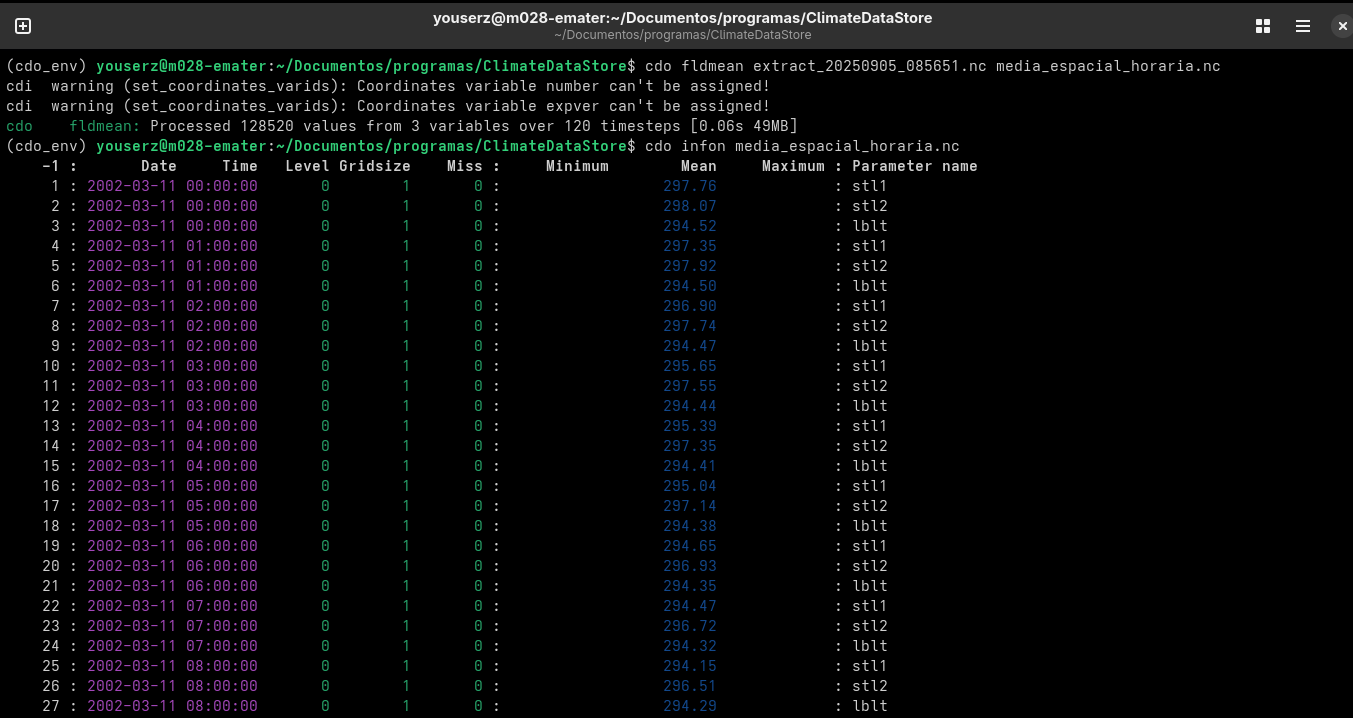
\includegraphics[width=0.8\textwidth]{1.png}
    \caption{Resultado do comando \texttt{fldmean} aplicado ao arquivo \texttt{output.nc}.}
    \label{fig:fldmean}
\end{figure}

\begin{itemize}
    \item \textbf{O que faz:} calcula a \textbf{média espacial} de todas as grades da variável ao longo da área definida no arquivo.
    \item \textbf{Exemplo:} se \texttt{output.nc} contém temperatura a 2 m (\texttt{t2m}) em toda a América do Sul, \texttt{fldmean} gera uma série temporal da temperatura média da região.
    \item \textbf{Resultado:} o arquivo \texttt{media\_espacial\_horaria.nc} tem \textbf{1 valor por timestep}, reduzindo drasticamente o tamanho do arquivo e facilitando análises temporais.
\end{itemize}

O comando a seguir exibe informações sobre o novo arquivo:

\begin{lstlisting}[language=bash]
cdo infon media_espacial_horaria.nc
\end{lstlisting}

\subsection{Média Diária (\texttt{daymean})}

\begin{lstlisting}[language=bash]
cdo daymean -mergetime output.nc teste_medial.nc
\end{lstlisting}

\begin{figure}[h!]
    \centering
    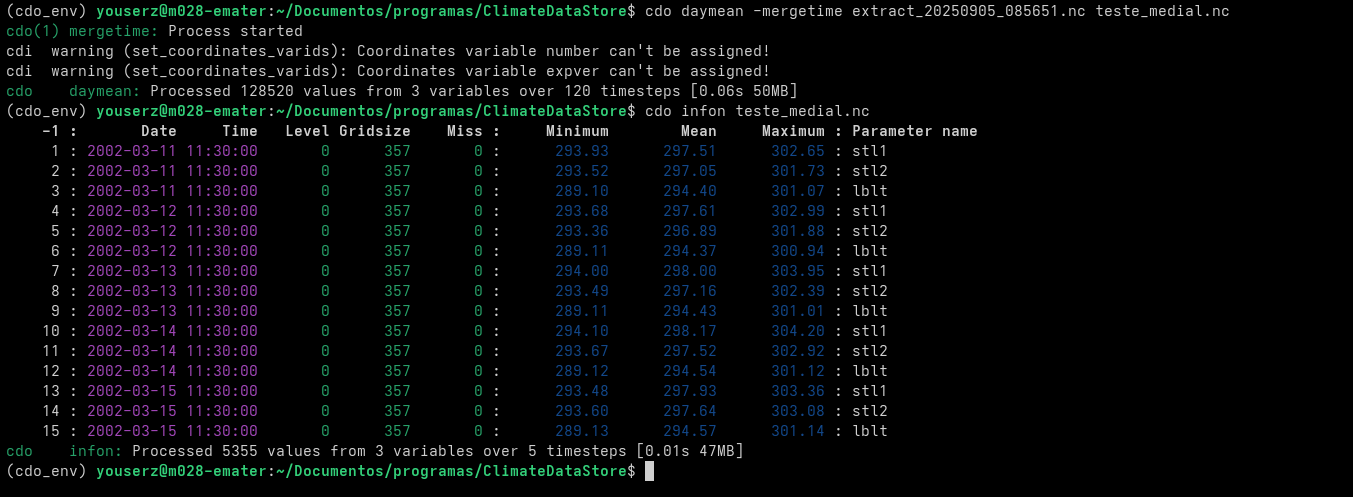
\includegraphics[width=0.8\textwidth]{2.png}
    \caption{Resultado do comando \texttt{daymean} após combinar timesteps horários.}
    \label{fig:daymean}
\end{figure}

\begin{itemize}
    \item \textbf{O que faz:} calcula a \textbf{média diária} a partir de dados horários.
    \item \texttt{-mergetime}: combina vários arquivos ou timesteps em uma sequência contínua antes de calcular a média diária.
    \item \textbf{Exemplo:} dados horários de temperatura ao longo de um mês se tornam uma série de médias diárias.
    \item \textbf{Resultado:} o arquivo \texttt{teste\_medial.nc} contém \textbf{1 valor por dia} para cada variável.
\end{itemize}

\subsection{Conversão de Unidades (\texttt{subc})}

\begin{lstlisting}[language=bash]
cdo subc,273.15 teste_medial.nc teste_medial1.nc
\end{lstlisting}

\begin{figure}[h!]
    \centering
    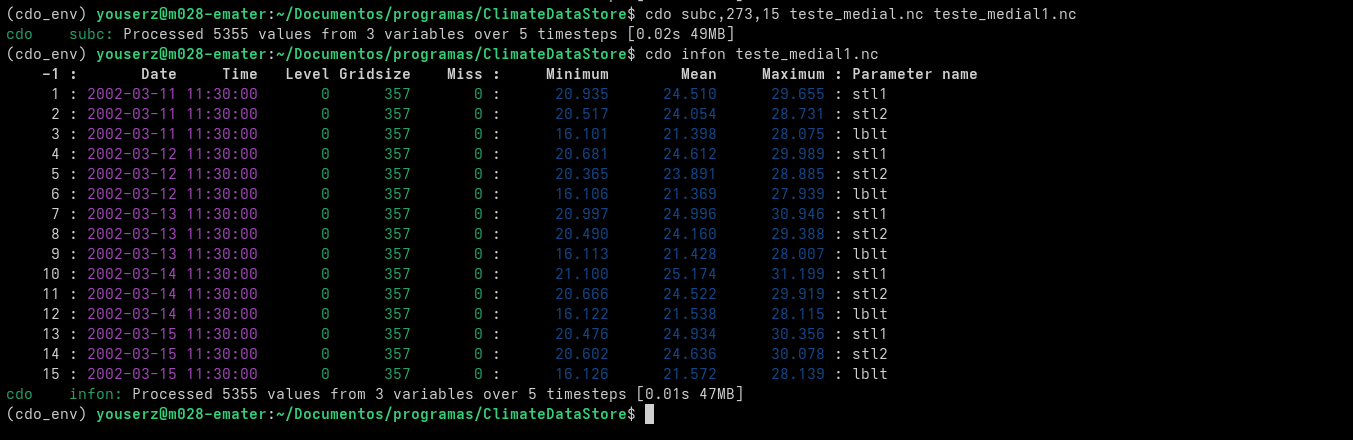
\includegraphics[width=0.8\textwidth]{3.png}
    \caption{Arquivo \texttt{teste\_medial1.nc} convertido de Kelvin para Celsius.}
    \label{fig:subc}
\end{figure}

\begin{itemize}
    \item \textbf{O que faz:} subtrai 273.15 de todos os valores, convertendo temperatura de Kelvin para Celsius.
    \item \textbf{Exemplo:} \texttt{t2m} passa de 297 K $\to$ 24 °C.
    \item \textbf{Resultado:} \texttt{teste\_medial1.nc} está pronto para análises e visualizações em unidades mais intuitivas.
\end{itemize}

\subsection{Observações Importantes}

\begin{itemize}
    \item Sempre \textbf{crie um novo arquivo} ao aplicar operações para evitar erros de permissão ou sobrescrita.
    \item É possível combinar várias operações em um \textbf{pipeline CDO}, reduzindo a quantidade de arquivos intermediários:
\end{itemize}
\begin{figure}[h!]
    \centering
    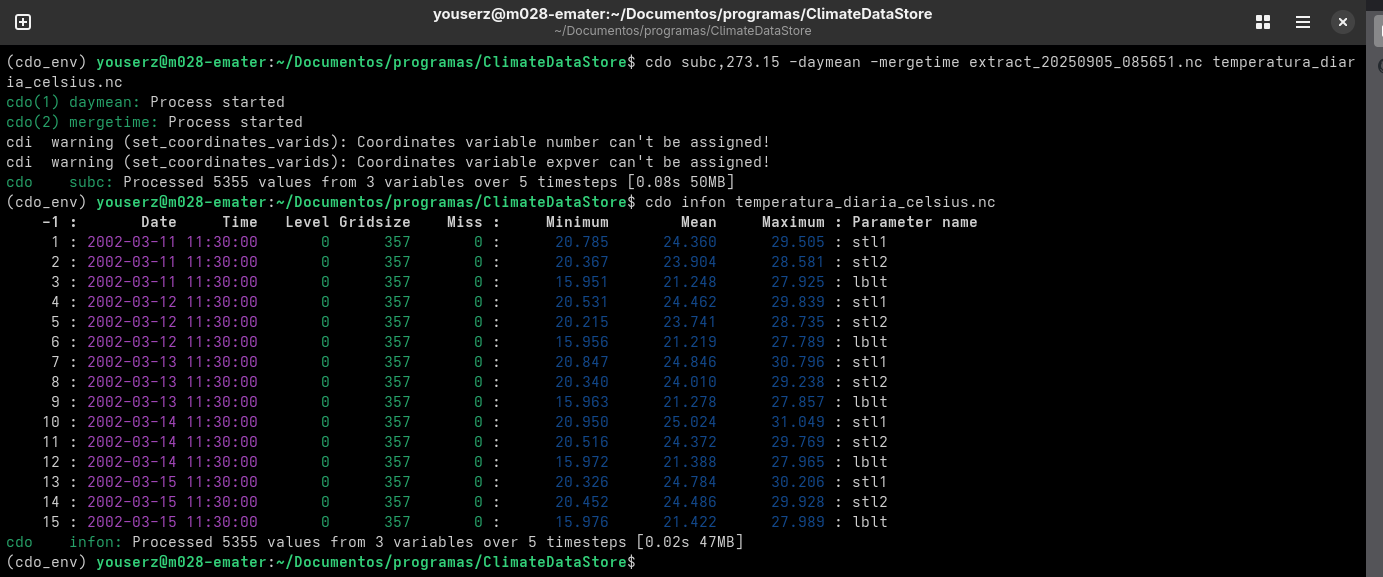
\includegraphics[width=0.8\textwidth]{4.png}
    \caption{Combinação das operções.}
    \label{fig:subc}
\end{figure}
\begin{lstlisting}[language=bash]
cdo subc,273.15 -daymean -mergetime output.nc temperatura_diaria_celsius.nc
\end{lstlisting}

Neste exemplo, o CDO executa as seguintes operações em sequência:

\begin{enumerate}
    \item Junta os timesteps (\texttt{mergetime}).
    \item Calcula a média diária (\texttt{daymean}).
    \item Converte de Kelvin para Celsius (\texttt{subc}).
    \item Salva o resultado em \texttt{temperatura\_diaria\_celsius.nc}.
\end{enumerate}


\end{document}


O projeto está bem documentado e o processo de configuração é direto.
